\documentclass[aspectratio=169]{beamer}

\usetheme{default}
\setbeamertemplate{navigation symbols}{}

%% ─── Packages ────────────────────────────────────────────────
\usepackage{amsmath,amssymb}
\usepackage{xcolor}
\usepackage{varwidth}
\usepackage{tikz}
\usepackage{adjustbox}
\usetikzlibrary{positioning,calc,arrows.meta}

\usepackage[n, advantage, operators, sets, adversary,
            probability, notions, logic, ff, mm, primitives,
            events, complexity, oracles, asymptotics, keys]{cryptocode}
\usepackage{hyperref}

%% ─── Colors ──────────────────────────────────────────────────
\definecolor{boxbordercolor}{HTML}{000000}
\definecolor{boxbgcolor}{HTML}{FFFFFF}
\definecolor{commentcolor}{HTML}{666666}
\definecolor{signalblue}{HTML}{3A76F0}
\definecolor{signalgreen}{HTML}{2A7B7B}
\definecolor{signalolive}{HTML}{4E7F60}
\hypersetup{
  colorlinks=true,
  linkcolor=signalblue,
  urlcolor=signalblue,
  citecolor=signalolive
}

%% ─── Signal-style pill for derived keys ──────────────────────
\newcommand{\keypill}[1]{%
  \tikz[baseline=(pill.base)]{%
    \node[fill=signalblue, text=white, rounded corners=4pt,
          inner xsep=4pt, inner ysep=1.5pt, font=\small\sffamily]
      (pill) {#1};%
  }%
}

%% ─── Signal-style pill for CKA algorithm names ─────────────
\newcommand{\algopill}[1]{%
  \tikz[baseline=(pill.base)]{%
    \node[fill=signalolive, text=white, rounded corners=4pt,
          inner xsep=4pt, inner ysep=1.5pt, font=\small\sffamily]
      (pill) {#1};%
  }%
}

%% ─── Red pill for state compromise ───────────────────────────
\definecolor{compromisered}{HTML}{CC2936}
\newcommand{\comppill}[1]{%
  \tikz[baseline=(pill.base)]{%
    \node[fill=compromisered, text=white, rounded corners=4pt,
          inner xsep=4pt, inner ysep=1.5pt, font=\small\sffamily]
      (pill) {#1};%
  }%
}

%% ─── Generic helpers ─────────────────────────────────────────
\newcommand{\calA}{\mathcal{A}}
\newcommand{\mycomment}[1]{\textcolor{commentcolor}{\small\textsl{// #1}}}

%% ─── codebox / titlecodebox ─────────────────────────────────
\newcommand{\codebox}[1]{%
    \begin{varwidth}{\linewidth}%
        \upshape%
        \begin{tabbing}%
            ~~~\=\quad\=\quad\=\quad\=\kill
            #1
        \end{tabbing}%
    \end{varwidth}%
}

\newcommand{\titlecodebox}[2]{%
    \sbox0{\codebox{#2}}%
    \sbox1{#1}%
    \fboxsep=0pt%
    \fcolorbox{boxbordercolor}{boxbgcolor}{%
        \begin{tabular}{@{}l@{}}
            \fboxsep=3pt%
            \colorbox{boxbordercolor!10!boxbgcolor}{%
                \makebox[\ifdim\wd0>\wd1 \wd0\else\wd1\fi][l]{#1}%
            } \\[-0.4pt]
            \usebox0
        \end{tabular}%
    }%
}

%% ─── constructionbox (titled bordered box) ──────────────────
\newcommand{\constructionbox}[2]{%
    \fboxsep=0pt%
    \fcolorbox{boxbordercolor}{boxbgcolor}{%
        \begin{minipage}{\dimexpr\linewidth-2\fboxrule\relax}%
            \fboxsep=8pt%
            \colorbox{boxbordercolor!10!boxbgcolor}{%
                \makebox[\dimexpr\linewidth-2\fboxsep\relax][l]{\textbf{#1}}%
            }\\[-0.4pt]
            \vspace{10pt}%
            \hspace{8pt}%
            \begin{minipage}{\dimexpr\linewidth-16pt\relax}%
                #2%
            \end{minipage}%
            \vspace{-2pt}%
        \end{minipage}%
    }%
}

%% ─── ScaledBox (scale content to fit) ───────────────────────
\newcommand{\ScaledBox}[2]{%
  \begin{adjustbox}{max width=\linewidth,max totalheight=#1,keepaspectratio}
    \begin{minipage}{\linewidth}
      #2
    \end{minipage}
  \end{adjustbox}
}

%% ─── CKA algorithm commands ─────────────────────────────────
\newcommand{\CKA}{\ensuremath{\mathsf{CKA}}}
\newcommand{\CKAInitKeyGen}{\ensuremath{\mathsf{Init\mbox{-}KeyGen}}}
\newcommand{\CKAInitA}{\ensuremath{\mathsf{Init\mbox{-}A}}}
\newcommand{\CKAInitB}{\ensuremath{\mathsf{Init\mbox{-}B}}}
\newcommand{\CKASendA}{\ensuremath{\mathsf{Send\mbox{-}A}}}
\newcommand{\CKARecB}{\ensuremath{\mathsf{Rec\mbox{-}B}}}
\newcommand{\CKASendB}{\ensuremath{\mathsf{Send\mbox{-}B}}}
\newcommand{\CKARecA}{\ensuremath{\mathsf{Rec\mbox{-}A}}}

%% ─── CKA Definition Box (Def 2.10) ─────────────────────────
%% Two versions: with informal descriptions (intro slide) and without (later)
\newcommand{\CKADefinitionBox}{%
  \constructionbox{Definition 2.10\quad (CKA)}{%
    \vspace{0.2cm}
    \procedure[linenumbering=false]{}{%
      \pclinecomment{generate shared key material} \\
      \CKAInitKeyGen(1^\lambda) \overset{\$}{\to} \mathsf{I}_{\mathsf{CKA}} \\ 
      \pclinecomment{\bf Party A} \\
      \pclinecomment{\bf initialize local state} \\
      \CKAInitA(\mathsf{I}_{\mathsf{CKA}}) \overset{\$}{\to} \mathsf{st}_\mathsf{A} \\
      \pclinecomment{} \\
      \CKASendA(\mathsf{st}_\mathsf{A}) \overset{\$}{\to} (\mathsf{K},\, \rho,\, \mathsf{st}_\mathsf{A}) \\
      \pclinecomment{receive $\rho$, derive matching key} \\
      \CKARecA(\mathsf{st}_\mathsf{A},\, \rho) \to (\mathsf{K},\, \mathsf{st}_\mathsf{A}) \\ \\
      \pclinecomment{\bf Party B} \\
      \pclinecomment{initialize local state from shared key} \\
      \CKAInitB(\mathsf{I}_{\mathsf{CKA}}) \overset{\$}{\to} \mathsf{st}_\mathsf{B} \\
      \pclinecomment{receive $\rho$, derive matching key} \\
      \CKARecB(\mathsf{st}_\mathsf{B},\, \rho) \to (\mathsf{K},\, \mathsf{st}_\mathsf{B}) \\
      \pclinecomment{produce fresh key, update state, send $\rho$} \\
      \CKASendB(\mathsf{st}_\mathsf{B}) \overset{\$}{\to} (\mathsf{K},\, \rho,\, \mathsf{st}_\mathsf{B})
    }
  }%
}

%% ─── CKA Protocol Box (Alice ↔ Bob interaction) ────────────
\newcommand{\CKAProtocolBox}{%
    \begin{varwidth}{20cm}%
    \pseudocodeblock{
      %% --- Header ---
      \textbf{Alice}(\mathsf{I}_{\mathsf{CKA}}) \< \< \textbf{Bob}(\mathsf{I}_{\mathsf{CKA}}) \\[0.1\baselineskip][\hline]
      \<\< \\[-0.5\baselineskip]
      %% --- Initialization ---
      \pclinecomment{generate initial state} \<\< \pclinecomment{generate initial state} \\[-0.1\baselineskip]
      \mathsf{st}_\mathsf{A} \gets \algopill{$\CKAInitA(\mathsf{I}_{\mathsf{CKA}})$} \<\< \mathsf{st}_\mathsf{B} \gets \algopill{$\CKAInitB(\mathsf{I}_{\mathsf{CKA}})$} \\[0.2\baselineskip]
   %
      %% --- Round 1: Alice sends, Bob receives (K1) ---
      \pclinecomment{generate new key and message} \<\< \\[-0.1\baselineskip]
      (\keypill{$\mathsf{K}_1$},\, \rho_1,\, \mathsf{st}_\mathsf{A}) \gets \algopill{$\CKASendA(\mathsf{st}_\mathsf{A})$} \<\< \\[-1.3\baselineskip]
      \< \sendmessageright*[7.5cm]{\rho_1} \< \\[-0.8\baselineskip]
      \<\< \pclinecomment{derive shared key $\mathsf{K}_1$} \\[-0.1\baselineskip]
      \<\< (\keypill{$\mathsf{K}_1$},\, \mathsf{st}_\mathsf{B}) \gets \algopill{$\CKARecB(\mathsf{st}_\mathsf{B},\, \rho_1)$} \\[0.2\baselineskip]
      %% --- Round 2: Bob sends, Alice receives (K2) ---
      \<\< \pclinecomment{generate new key and message} \\[-0.1\baselineskip]
      \<\< (\keypill{$\mathsf{K}_2$},\, \rho_2,\, \mathsf{st}_\mathsf{B}) \gets \algopill{$\CKASendB(\mathsf{st}_\mathsf{B})$} \\\\[-1.8\baselineskip]
      \< \sendmessageleft*[7.5cm]{\rho_2} \< \\[-0.8\baselineskip]
      \pclinecomment{derive shared key $\mathsf{K}_2$} \<\< \\[-0.1\baselineskip]
      (\keypill{$\mathsf{K}_2$},\, \mathsf{st}_\mathsf{A}) \gets \algopill{$\CKARecA(\mathsf{st}_\mathsf{A},\, \rho_2)$} \\[0.2\baselineskip]
      %% --- Round 3: Alice sends, Bob receives (K3) [overlay] ---
      \onslide<2->{\pclinecomment{generate new key and message}} \<\< \\[-0.1\baselineskip]
      \onslide<2->{(\keypill{$\mathsf{K}_3$},\, \rho_3,\, \mathsf{st}_\mathsf{A}) \gets \algopill{$\CKASendA(\mathsf{st}_\mathsf{A})$}} \<\< \\[-1.3\baselineskip]
      \< \onslide<2->{\sendmessageright*[7.5cm]{\rho_3}} \< \\[-0.8\baselineskip]
      \<\< \onslide<2->{\pclinecomment{derive shared key $\mathsf{K}_3$}} \\[-0.1\baselineskip]
      \<\< \onslide<2->{(\keypill{$\mathsf{K}_3$},\, \mathsf{st}_\mathsf{B}) \gets \algopill{$\CKARecB(\mathsf{st}_\mathsf{B},\, \rho_3)$}} \\[0.2\baselineskip]
      %% --- Round 4: Bob sends, Alice receives (K4) [overlay] ---
      \<\< \onslide<2->{\pclinecomment{generate new key and message}} \\[-0.1\baselineskip]
      \<\< \onslide<2->{(\keypill{$\mathsf{K}_4$},\, \rho_4,\, \mathsf{st}_\mathsf{B}) \gets \algopill{$\CKASendB(\mathsf{st}_\mathsf{B})$}} \\\\[-1.8\baselineskip]
      \< \onslide<2->{\sendmessageleft*[7.5cm]{\rho_4}} \< \\[-0.8\baselineskip]
      \onslide<2->{\pclinecomment{derive shared key $\mathsf{K}_4$}} \<\< \\[-0.1\baselineskip]
      \onslide<2->{(\keypill{$\mathsf{K}_4$},\, \mathsf{st}_\mathsf{A}) \gets \algopill{$\CKARecA(\mathsf{st}_\mathsf{A},\, \rho_4)$}} \<\<
    }%
    \end{varwidth}%
}

%% ═════════════════════════════════════════════════════════════
%%  DOCUMENT
%% ═════════════════════════════════════════════════════════════
\begin{document}

%% ─── Slide 1: Protocol primitives overview ──────────────────
\begin{frame}[plain]
\centering
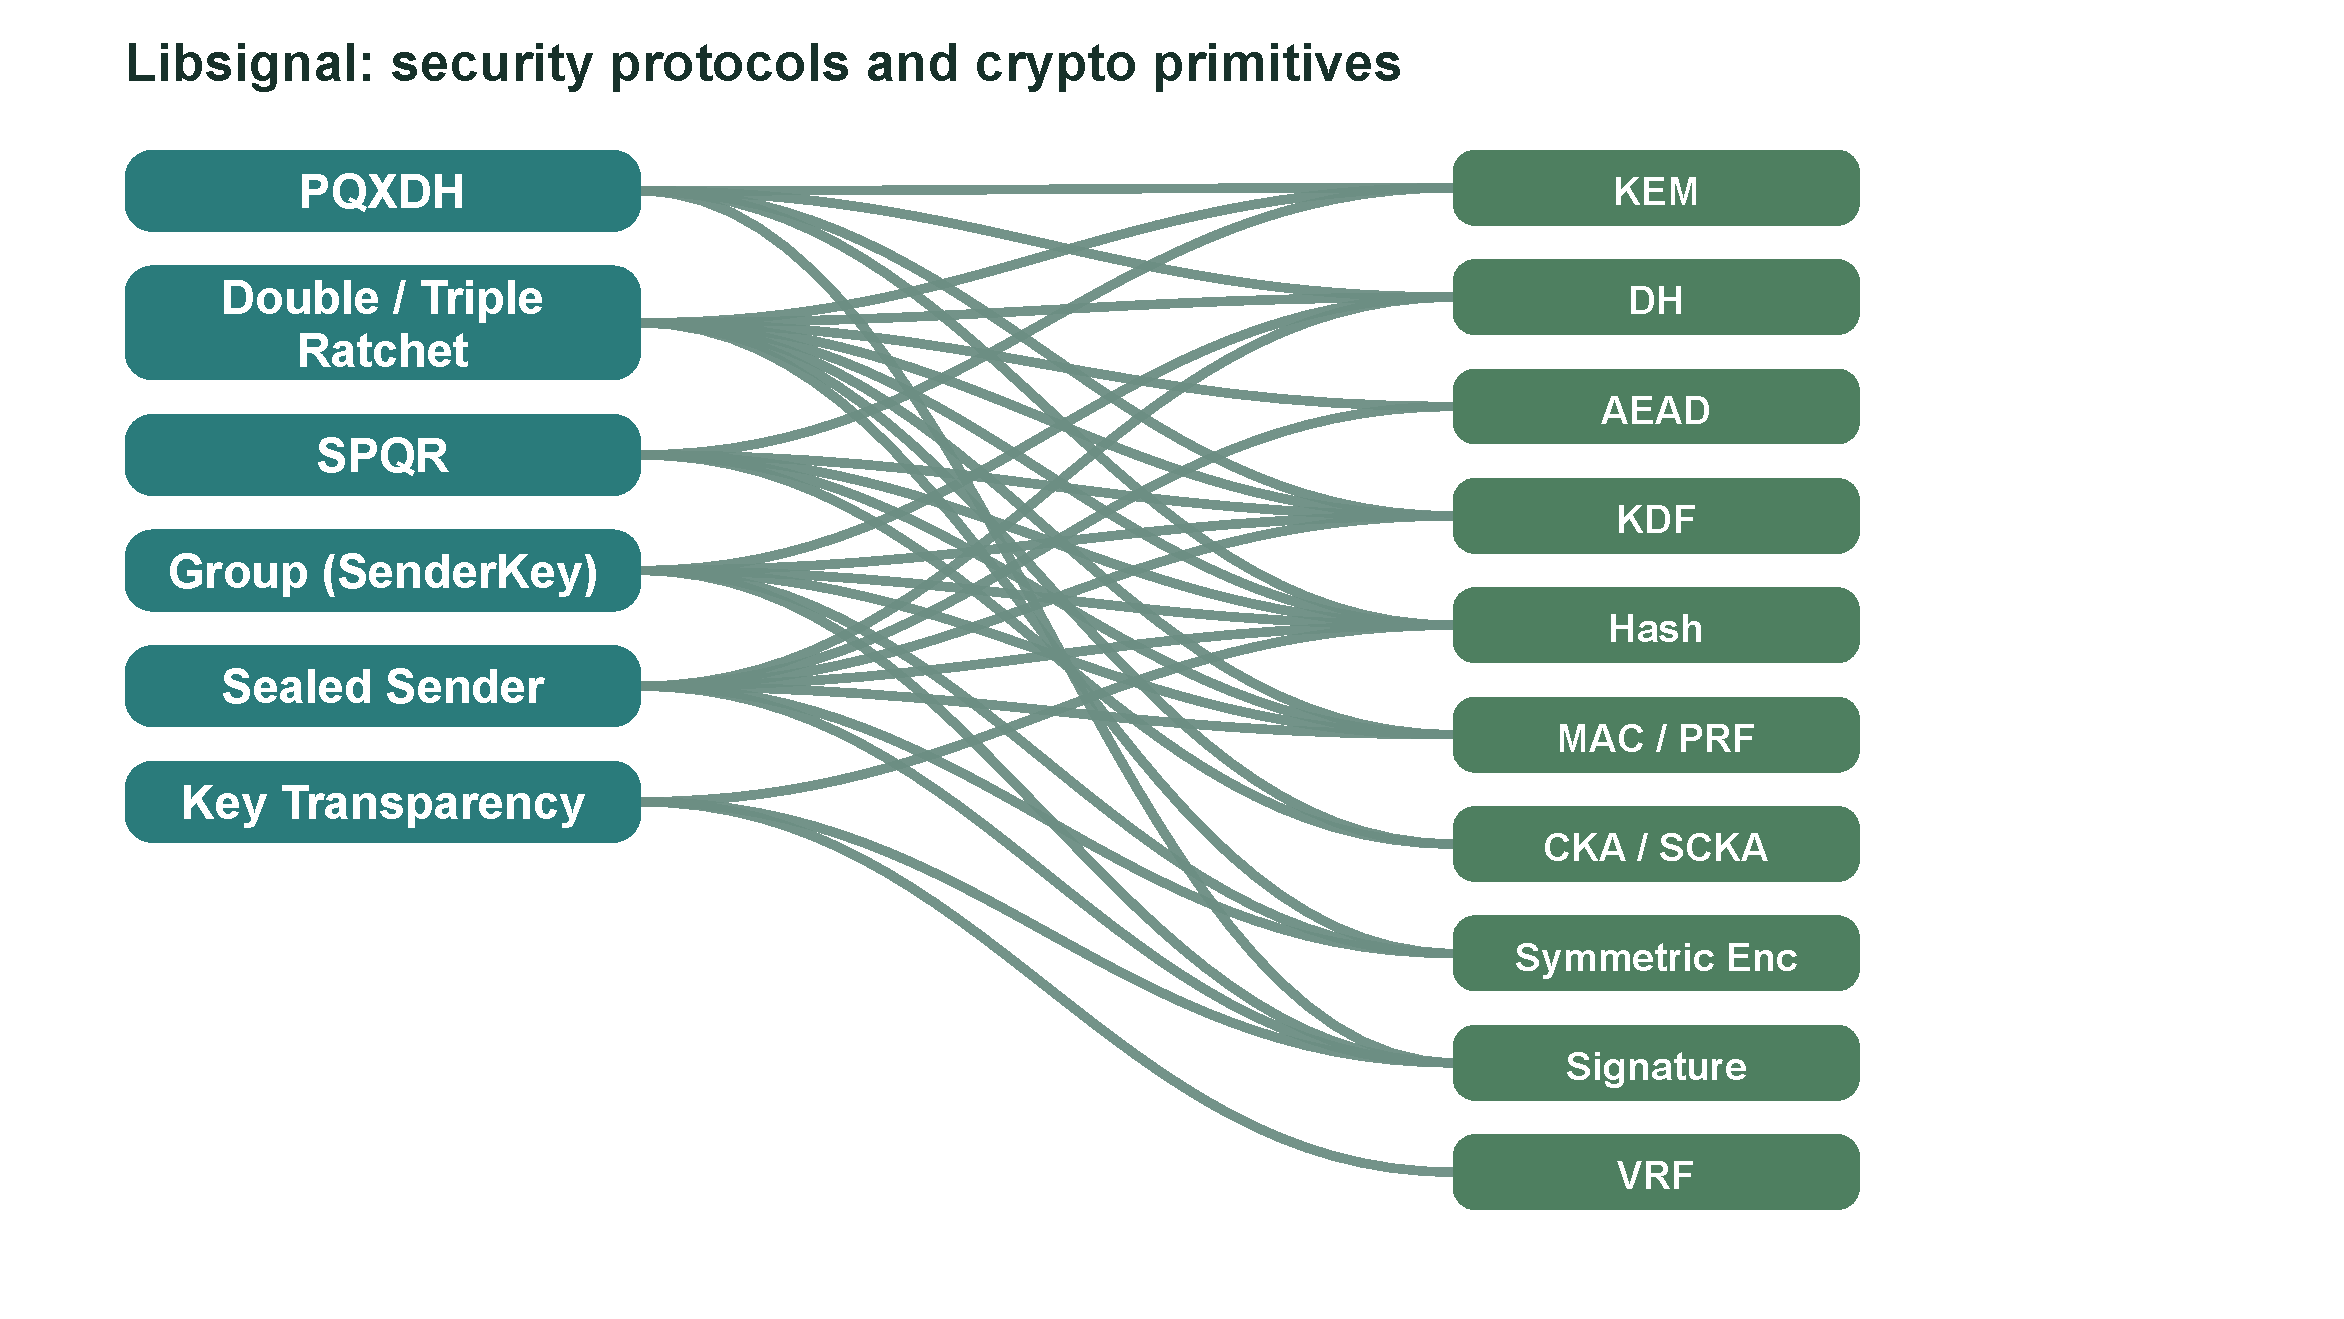
\includegraphics[width=0.94\paperwidth]{protocol_primitives_all.pdf}
\end{frame}

%% ─── Slide 2: CKA highlighted ──────────────────────────────
\begin{frame}[plain]
\centering
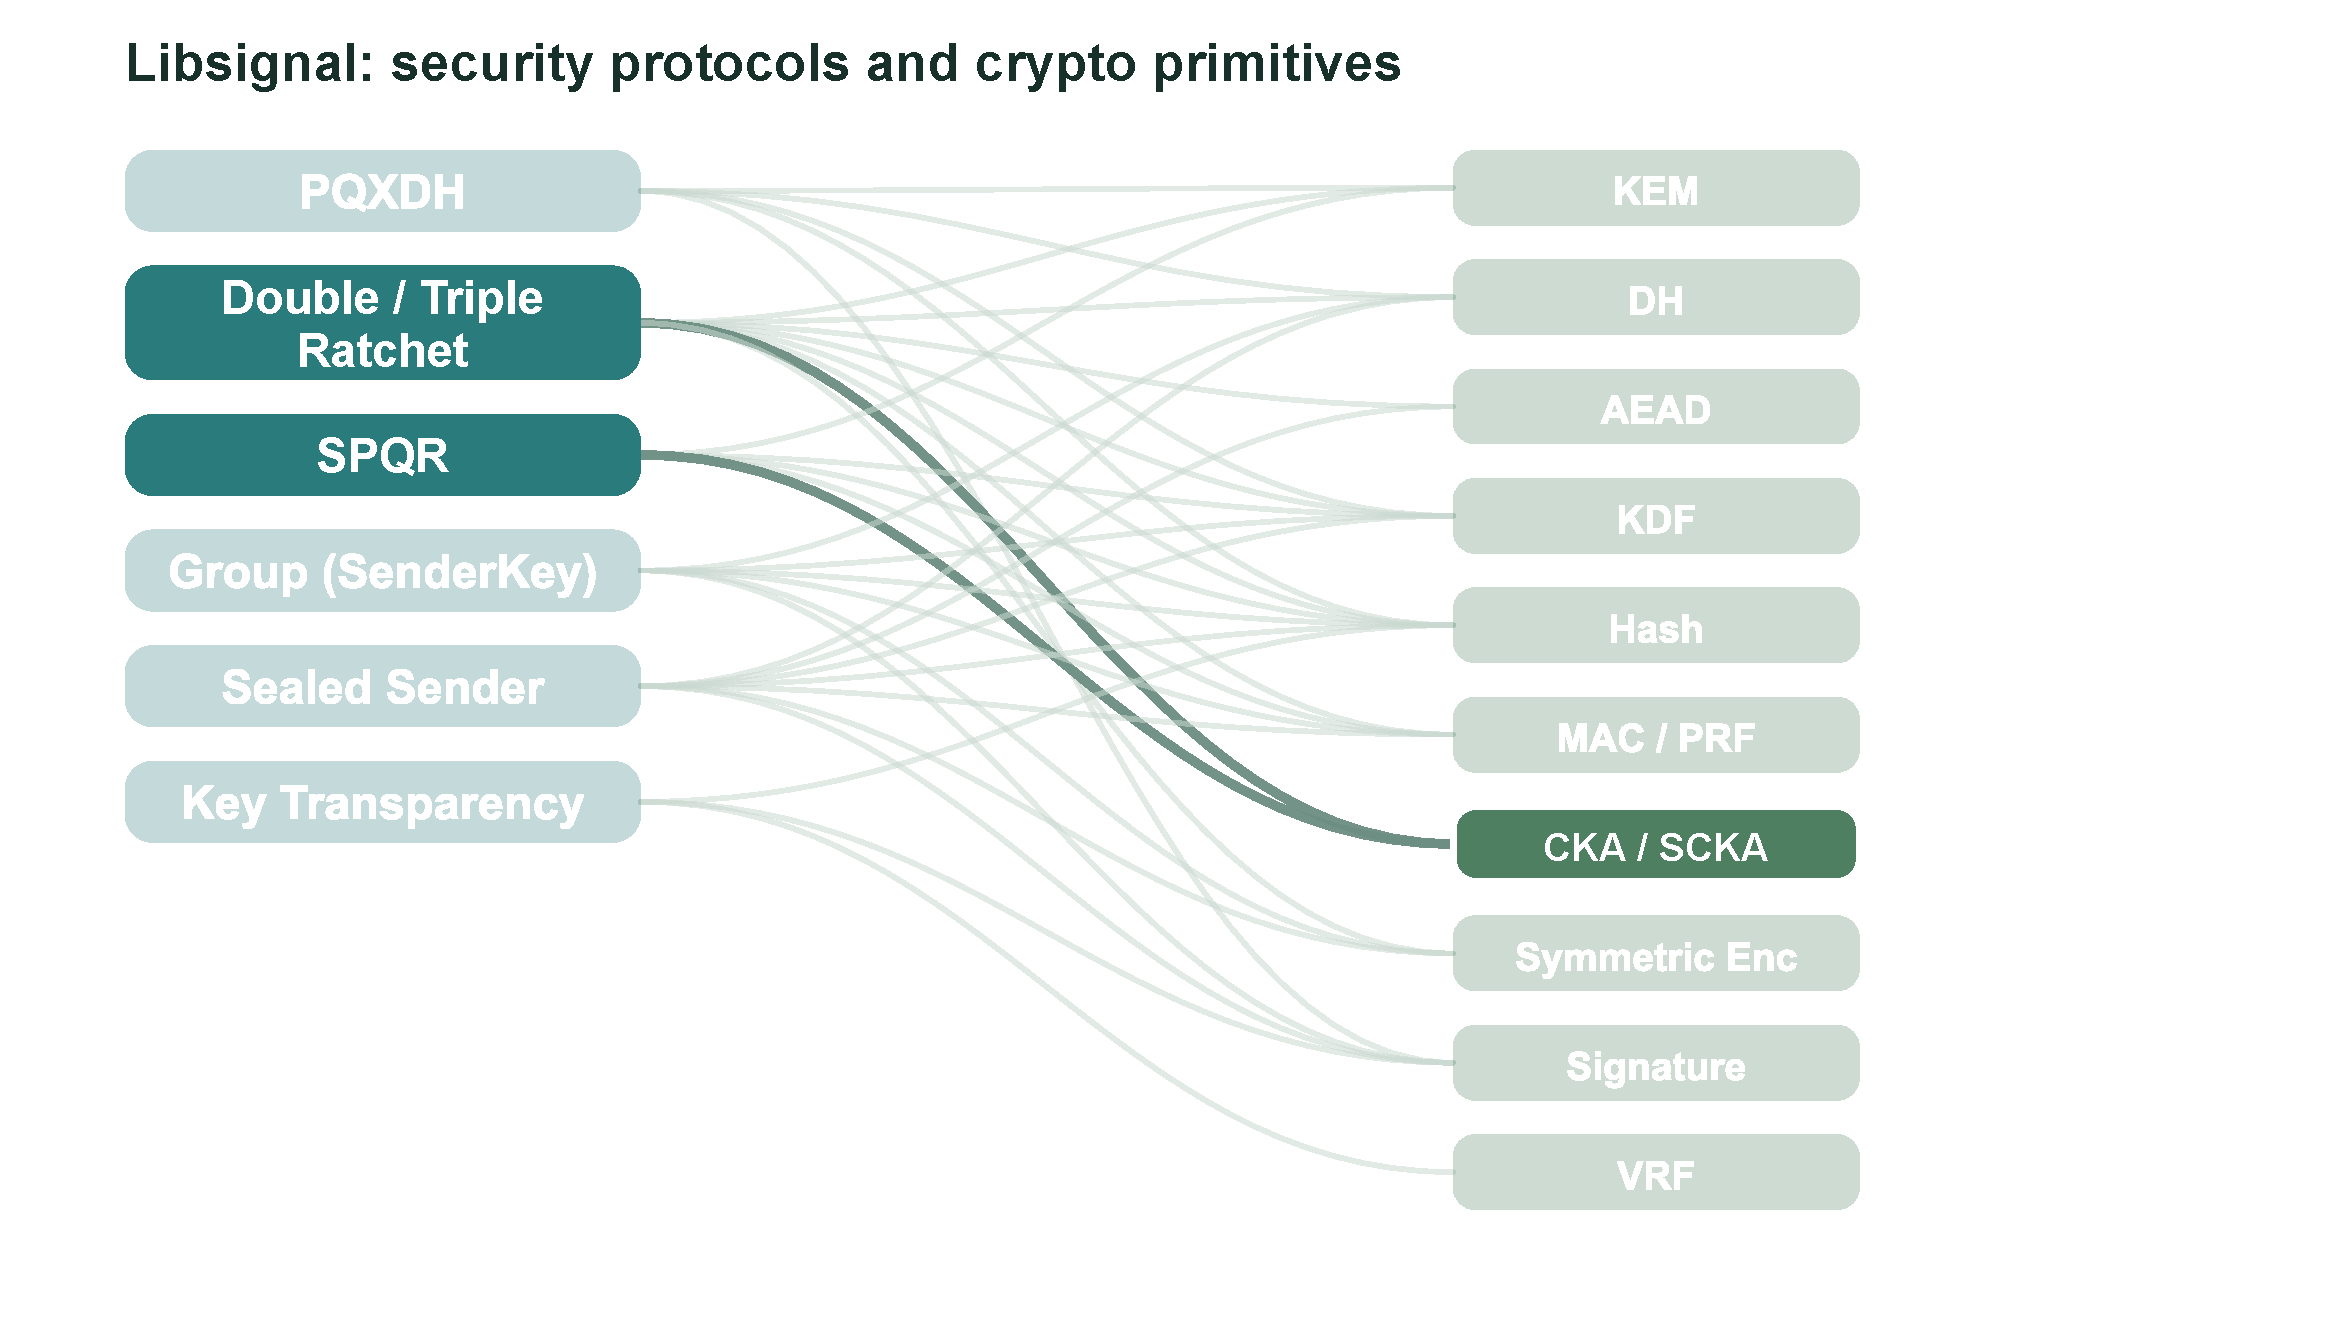
\includegraphics[width=0.94\paperwidth]{protocol_primitives_cka_selected.pdf}
\end{frame}

%% ─── Slide 3: CKA algorithm overview ─────────────────────────
\begin{frame}[t]{Continuous Key Agreement}
\medskip
\large
\begin{tabular}{@{}ll@{}}
  \algopill{$\textbf{A}$}\,,\;\algopill{$\textbf{B}$} & participating parties \\[0.4em]
  \multicolumn{2}{@{}l@{}}{\textcolor{signalblue}{\rule{\linewidth}{1.5pt}}} \\[0.4em]
  \algopill{$\CKAInitKeyGen$} & generate shared initial key material \\[0.6em]
  \algopill{$\CKAInitA$}\,,\;\algopill{$\CKAInitB$} & initialize local party state from shared key \\[0.6em]
  \algopill{$\CKASendA$}\,,\;\algopill{$\CKASendB$} & produce a fresh key, output message, update state \\[0.6em]
  \algopill{$\CKARecA$}\,,\;\algopill{$\CKARecB$} & receive message, derive shared key, update state \\[0.6em]
\end{tabular}
\end{frame}

%% ─── Slide 4–6: CKA protocol (centered) ─────────────────────
\begin{frame}[plain]
\vspace*{0.025cm}
\hspace*{-0.5cm}
\centering
%\onslide<2->{%
\begin{adjustbox}{max width=1.05\linewidth,max totalheight=1.\textheight,keepaspectratio}
\CKAProtocolBox
\end{adjustbox}%
%}
\end{frame}

%% ─── Slide: State compromise illustration ───────────────────
\begin{frame}[plain]
\vspace*{0.025cm}
\hspace*{-0.5cm}
\centering
\begin{adjustbox}{max width=1.05\linewidth,max totalheight=1.\textheight,keepaspectratio}
\begin{varwidth}{20cm}%
\pseudocodeblock{
  %% --- Header ---
  \textbf{Alice}(\mathsf{I}_{\mathsf{CKA}}) \< \< \textbf{Bob}(\mathsf{I}_{\mathsf{CKA}}) \\[0.1\baselineskip][\hline]
  \<\< \\[-0.5\baselineskip]
  %% --- Initialization ---
  \pclinecomment{generate initial state} \<\< \pclinecomment{generate initial state} \\[-0.1\baselineskip]
  \mathsf{st}_\mathsf{A} \gets \algopill{$\CKAInitA(\mathsf{I}_{\mathsf{CKA}})$} \<\< \mathsf{st}_\mathsf{B} \gets \algopill{$\CKAInitB(\mathsf{I}_{\mathsf{CKA}})$} \\[0.2\baselineskip]
  %% --- Round 1: K1 — Bob compromised ---
  \pclinecomment{generate new key and message} \<\< \\[-0.1\baselineskip]
  (\keypill{$\mathsf{K}_1$},\, \rho_1,\, \mathsf{st}_\mathsf{A}) \gets \algopill{$\CKASendA(\mathsf{st}_\mathsf{A})$} \<\< \\[-1.3\baselineskip]
  \< \sendmessageright*[7.5cm]{\rho_1} \< \\[-0.8\baselineskip]
  \<\< \pclinecomment{derive shared key $\mathsf{K}_1$} \\[-0.1\baselineskip]
  \<\< \comppill{$(\mathsf{K}_1,\, \mathsf{st}_\mathsf{B}) \gets \CKARecB(\mathsf{st}_\mathsf{B},\, \rho_1)$} \\[0.2\baselineskip]
  %% --- Round 2: K2 ---
  \<\< \pclinecomment{generate new key and message} \\[-0.1\baselineskip]
  \<\< (\keypill{$\mathsf{K}_2$},\, \rho_2,\, \mathsf{st}_\mathsf{B}) \gets \algopill{$\CKASendB(\mathsf{st}_\mathsf{B})$} \\\\[-1.8\baselineskip]
  \< \sendmessageleft*[7.5cm]{\rho_2} \< \\[-0.8\baselineskip]
  \pclinecomment{derive shared key $\mathsf{K}_2$} \<\< \\[-0.1\baselineskip]
  (\keypill{$\mathsf{K}_2$},\, \mathsf{st}_\mathsf{A}) \gets \algopill{$\CKARecA(\mathsf{st}_\mathsf{A},\, \rho_2)$} \\[0.2\baselineskip]
  %% --- Round 3: K3 — Alice compromised ---
  \pclinecomment{generate new key and message} \<\< \\[-0.1\baselineskip]
  \comppill{$(\mathsf{K}_3,\, \rho_3,\, \mathsf{st}_\mathsf{A}) \gets \CKASendA(\mathsf{st}_\mathsf{A})$} \<\< \\[-1.3\baselineskip]
  \< \sendmessageright*[7.5cm]{\rho_3} \< \\[-0.8\baselineskip]
  \<\< \pclinecomment{derive shared key $\mathsf{K}_3$} \\[-0.1\baselineskip]
  \<\< (\keypill{$\mathsf{K}_3$},\, \mathsf{st}_\mathsf{B}) \gets \algopill{$\CKARecB(\mathsf{st}_\mathsf{B},\, \rho_3)$} \\[0.2\baselineskip]
  %% --- Round 4: K4 ---
  \<\< \pclinecomment{generate new key and message} \\[-0.1\baselineskip]
  \<\< (\keypill{$\mathsf{K}_4$},\, \rho_4,\, \mathsf{st}_\mathsf{B}) \gets \algopill{$\CKASendB(\mathsf{st}_\mathsf{B})$} \\\\[-1.8\baselineskip]
  \< \sendmessageleft*[7.5cm]{\rho_4} \< \\[-0.8\baselineskip]
  \pclinecomment{derive shared key $\mathsf{K}_4$} \<\< \\[-0.1\baselineskip]
  (\keypill{$\mathsf{K}_4$},\, \mathsf{st}_\mathsf{A}) \gets \algopill{$\CKARecA(\mathsf{st}_\mathsf{A},\, \rho_4)$} \<\<
}%
\end{varwidth}%
\end{adjustbox}%
\end{frame}

%% ─── Slide: CKA Security Game (adapted from [ACD20] Fig. 3) ──
\newcommand{\CKASecurityGameBox}{%
  \constructionbox{Security Game for CKA\quad{\small\normalfont Def.~13 from \href{https://eprint.iacr.org/2018/1037.pdf}{[ACD19, \emph{The Double Ratchet}]}}}{%
    \vspace{0.2cm}
    \begin{pchstack}[space=0.4em]
      %% --- Column 1: O-Init + O-Corr-A + O-Corr-B ---
      \begin{pcvstack}[space=0.3cm]
        \procedure[linenumbering=false]{$\textcolor{signalolive}{\textbf{O\mbox{-}Init}}(t^*)$}{%
          \mathsf{I}_{\mathsf{CKA}} \overset{\$}{\gets} \CKAInitKeyGen(1^\lambda) \\
          \mathsf{st}_\mathsf{A} \gets \CKAInitA(\mathsf{I}_{\mathsf{CKA}}) \\
          \mathsf{st}_\mathsf{B} \gets \CKAInitB(\mathsf{I}_{\mathsf{CKA}}) \\
          t_\mathsf{A},\, t_\mathsf{B} \gets 0 \\
          b \overset{\$}{\gets} \{0,1\}
        }
        \onslide<2->{%
        \pcvspace \pcvspace
        \procedure[linenumbering=false]{$\textcolor{compromisered}{\textbf{O\mbox{-}Corr\mbox{-}A}}$}{%
          \textbf{req } \textsf{allow-corr} \text{ or } \textsf{finished}_\mathsf{A} \\
          \textbf{return } \mathsf{st}_\mathsf{A}
        }
        \procedure[linenumbering=false]{$\textcolor{compromisered}{\textbf{O\mbox{-}Corr\mbox{-}B}}$}{%
          \textbf{req } \textsf{allow-corr} \text{ or } \textsf{finished}_\mathsf{B} \\
          \textbf{return } \mathsf{st}_\mathsf{B}
        }
        }% end onslide<2->
        \onslide<4->{%
        \procedure[linenumbering=false]{$\textcolor{compromisered}{\textbf{Win}_{\calA}}$}{%
          b' \gets \calA^{\mathcal{O}} \\
          \textbf{return } (b' = b)
        }
        }% end onslide<4->
      \end{pcvstack}
      %% --- Column 2: A oracles ---
      \begin{pcvstack}[space=0.3cm]
        \procedure[linenumbering=false]{$\textcolor{signalolive}{\textbf{O\mbox{-}Send\mbox{-}A}}$}{%
          t_\mathsf{A} \mathrel{++} \\
          (\mathsf{K}_{t_\mathsf{A}},\, \rho_{t_\mathsf{A}},\, \mathsf{st}_\mathsf{A}) \overset{\$}{\gets} \CKASendA(\mathsf{st}_\mathsf{A}) \\
          \textbf{return } (\rho_{t_\mathsf{A}},\, \mathsf{K}_{t_\mathsf{A}})
        }
        \procedure[linenumbering=false]{$\textcolor{signalolive}{\textbf{O\mbox{-}Rec\mbox{-}A}}$}{%
          t_\mathsf{A} \mathrel{++} \\
          (\mathsf{K}_{t_\mathsf{A}},\, \mathsf{st}_\mathsf{A}) \gets \CKARecA(\mathsf{st}_\mathsf{A},\, \rho_{t_\mathsf{A}})
        }
        \onslide<3->{%
        \procedure[linenumbering=false]{$\textcolor{signalblue}{\textbf{O\mbox{-}Chall\mbox{-}A}}$}{%
          t_\mathsf{A} \mathrel{++} \\
          \textbf{req } t_\mathsf{A} = t^* \\
          (\mathsf{K}_{t_\mathsf{A}},\, \rho_{t_\mathsf{A}},\, \mathsf{st}_\mathsf{A}) \overset{\$}{\gets} \CKASendA(\mathsf{st}_\mathsf{A}) \\
          \textbf{if } b = 0 \\
          \t \textbf{return } (\rho_{t_\mathsf{A}},\, \mathsf{K}_{t_\mathsf{A}}) \\
          \textbf{else} \\
          \t \mathsf{K} \overset{\$}{\gets} \mathcal{K} \\
          \t \textbf{return } (\rho_{t_\mathsf{A}},\, \mathsf{K})
        }
        }% end onslide<3->
      \end{pcvstack}
      %% --- Column 3: B oracles ---
      \begin{pcvstack}[space=0.3cm]
        \procedure[linenumbering=false]{$\textcolor{signalolive}{\textbf{O\mbox{-}Send\mbox{-}B}}$}{%
          t_\mathsf{B} \mathrel{++} \\
          (\mathsf{K}_{t_\mathsf{B}},\, \rho_{t_\mathsf{B}},\, \mathsf{st}_\mathsf{B}) \overset{\$}{\gets} \CKASendB(\mathsf{st}_\mathsf{B}) \\
          \textbf{return } (\rho_{t_\mathsf{B}},\, \mathsf{K}_{t_\mathsf{B}})
        }
        \procedure[linenumbering=false]{$\textcolor{signalolive}{\textbf{O\mbox{-}Rec\mbox{-}B}}$}{%
          t_\mathsf{B} \mathrel{++} \\
          (\mathsf{K}_{t_\mathsf{B}},\, \mathsf{st}_\mathsf{B}) \gets \CKARecB(\mathsf{st}_\mathsf{B},\, \rho_{t_\mathsf{B}})
        }
        \onslide<3->{%
        \procedure[linenumbering=false]{$\textcolor{signalblue}{\textbf{O\mbox{-}Chall\mbox{-}B}}$}{%
          t_\mathsf{B} \mathrel{++} \\
          \textbf{req } t_\mathsf{B} = t^* \\
          (\mathsf{K}_{t_\mathsf{B}},\, \rho_{t_\mathsf{B}},\, \mathsf{st}_\mathsf{B}) \overset{\$}{\gets} \CKASendB(\mathsf{st}_\mathsf{B}) \\
          \textbf{if } b = 0 \\
          \t \textbf{return } (\rho_{t_\mathsf{B}},\, \mathsf{K}_{t_\mathsf{B}}) \\
          \textbf{else} \\
          \t \mathsf{K} \overset{\$}{\gets} \mathcal{K} \\
          \t \textbf{return } (\rho_{t_\mathsf{B}},\, \mathsf{K})
        }
        }% end onslide<3->
      \end{pcvstack}
    \end{pchstack}
    \onslide<2->{%
    \vspace{0.3cm}
    \centering
    $\textsf{allow-corr} \;:\Longleftrightarrow\; \max(t_\mathsf{A},\, t_\mathsf{B}) \le t^* - 2$
    \qquad
    $\textsf{finished}_\mathsf{P} \;:\Longleftrightarrow\; t_\mathsf{P} \ge t^* + \Delta_{\mathsf{CKA}}$
    }% end onslide<2->
  }%
}

\begin{frame}[plain]
\vspace*{0.1cm}
\hspace*{-0.5cm}%
\ScaledBox{0.98\textheight}{\CKASecurityGameBox}
%% --- TikZ overlay: oracle group labels (top-right) + Def.13 (bottom-right) ---
\begin{tikzpicture}[remember picture, overlay]
  %% Informal oracle group labels — appear with each overlay
  \onslide<1->{%
  \node[anchor=north east, font=\small\sffamily, text=signalolive]
    at ([xshift=-0.4cm, yshift=-1.3cm]current page.north east)
    {\textbf{communication oracles}};%
  }%
  \onslide<2->{%
  \node[anchor=north east, font=\small\sffamily, text=compromisered]
    at ([xshift=-0.4cm, yshift=-1.9cm]current page.north east)
    {\textbf{corruption oracles}};%
  }%
  \onslide<3->{%
  \node[anchor=north east, font=\small\sffamily, text=signalblue]
    at ([xshift=-0.4cm, yshift=-2.5cm]current page.north east)
    {\textbf{challenge oracles}};%
  }%
  %% Def.13 security definition — bottom-right
  \onslide<4->{%
  \node[anchor=south east, text width=4.8cm, align=left,
        fill=signalblue!8, draw=signalblue!40, rounded corners=3pt,
        inner sep=6pt, font=\small]
    at ([xshift=-0.3cm, yshift=0.4cm]current page.south east)
    {%
      \textbf{\underline{CKA Security against class $\cal C$}}\;:\\[4pt]
      $\forall \calA \in {\cal C}. \,\bigl|\Pr[\textsf{Win}_{\calA}] - \tfrac{1}{2}\bigr| \;\le\; \varepsilon$%
    };%
  }% end onslide<4->
\end{tikzpicture}
\end{frame}

%% ─── Slide: Generic CKA recall (rounds 1–2 only) ──────────────
\begin{frame}[plain]{CKA construction}
\vspace*{0.025cm}
\hspace*{-0.5cm}
\centering
\begin{adjustbox}{max width=1.05\linewidth,max totalheight=1.\textheight,keepaspectratio}
\begin{varwidth}{20cm}%
\pseudocodeblock{
  %% --- Header ---
  \textbf{Alice}(\mathsf{I}_{\mathsf{CKA}}) \< \< \textbf{Bob}(\mathsf{I}_{\mathsf{CKA}}) \\[0.1\baselineskip][\hline]
  \<\< \\[-0.5\baselineskip]
  %% --- Initialization ---
  \pclinecomment{generate initial state} \<\< \pclinecomment{generate initial state} \\[-0.1\baselineskip]
  \mathsf{st}_\mathsf{A} \gets \algopill{$\CKAInitA(\mathsf{I}_{\mathsf{CKA}})$} \<\< \mathsf{st}_\mathsf{B} \gets \algopill{$\CKAInitB(\mathsf{I}_{\mathsf{CKA}})$} \\[0.2\baselineskip]
  %% --- Round 1: Alice sends, Bob receives (K1) ---
  \pclinecomment{generate new key and message} \<\< \\[-0.1\baselineskip]
  (\keypill{$\mathsf{K}_1$},\, \rho_1,\, \mathsf{st}_\mathsf{A}) \gets \algopill{$\CKASendA(\mathsf{st}_\mathsf{A})$} \<\< \\[-1.3\baselineskip]
  \< \sendmessageright*[7.5cm]{\rho_1} \< \\[-0.8\baselineskip]
  \<\< \pclinecomment{derive shared key $\mathsf{K}_1$} \\[-0.1\baselineskip]
  \<\< (\keypill{$\mathsf{K}_1$},\, \mathsf{st}_\mathsf{B}) \gets \algopill{$\CKARecB(\mathsf{st}_\mathsf{B},\, \rho_1)$} \\[0.2\baselineskip]
  %% --- Round 2: Bob sends, Alice receives (K2) ---
  \<\< \pclinecomment{generate new key and message} \\[-0.1\baselineskip]
  \<\< (\keypill{$\mathsf{K}_2$},\, \rho_2,\, \mathsf{st}_\mathsf{B}) \gets \algopill{$\CKASendB(\mathsf{st}_\mathsf{B})$} \\\\[-1.8\baselineskip]
  \< \sendmessageleft*[7.5cm]{\rho_2} \< \\[-0.8\baselineskip]
  \pclinecomment{derive shared key $\mathsf{K}_2$} \<\< \\[-0.1\baselineskip]
  (\keypill{$\mathsf{K}_2$},\, \mathsf{st}_\mathsf{A}) \gets \algopill{$\CKARecA(\mathsf{st}_\mathsf{A},\, \rho_2)$} \<\<
}%
\end{varwidth}%
\end{adjustbox}%
\end{frame}

%% ─── Slide: Algebraic structure for DDH-based CKA ─────────────
\begin{frame}[t]{Diffie-Hellman group structure and DDH assumption}
\medskip
\large

Let $(G, +)$ be a cyclic group of prime order $q$, with generator $g$.

\medskip
We use the \textbf{scalar multiplication} $\mathbb{Z}_q \times G \to G$\,:

\medskip
\begin{center}
\begin{tabular}{@{}r@{\;:\;}l@{}}
  \algopill{$x \cdot g$} & compute $\underbrace{g + g + \cdots + g}_{x \text{ times}}$ \\[1em]
\end{tabular}
\end{center}

\medskip
\pause 
\medskip
\begin{tabular}{@{}ll@{}}
  \textbf{Associativity} & $x \cdot (y \cdot g) \;=\; (x \cdot y) \cdot g$ \\[0.6em]
  \textbf{Commutativity} & $x \cdot (y \cdot g) \;=\; y \cdot (x \cdot g)$ \\[0.6em]
  \multicolumn{2}{@{}l@{}}{\textcolor{signalolive}{$\longrightarrow$ \textsf{allow computing a shared key\;} }$(a{\cdot}b) \cdot g$} \\[0.4em]
  \pause
  \\[0.2em]
  \textbf{DDH assumption} & $(g,\; a{\cdot}g,\; b{\cdot}g,\;\underline{(a{\cdot}b) \cdot g}\;)\cong (g,\; a{\cdot}g,\; b{\cdot}g,\;\underline{r \cdot g}\;)$ \\[0.6em]
  \multicolumn{2}{@{}l@{}}{\textcolor{signalolive}{$\longrightarrow$ \textsf{allows proving security}}}
\end{tabular}

\end{frame}

%% ─── Slide: CKA from DDH construction (rounds 1–2) ───────────
\begin{frame}[plain]{CKA construction from DDH}
\vspace*{.05cm}
\hspace*{-0.5cm}
\centering
\begin{adjustbox}{max width=1.05\linewidth,max totalheight=1.\textheight,keepaspectratio}
\begin{varwidth}{20cm}%
\pseudocodeblock{
  %% --- Header ---
  \textbf{Alice}(\algopill{$\mathsf{I}_{\mathsf{CKA}} = (h,\, x_0)$}) \< \algopill{$h = x_0 \cdot g$}\< \textbf{Bob}(\algopill{$\mathsf{I}_{\mathsf{CKA}} = (h,\, x_0)$}) \\[0.1\baselineskip][\hline]
  \<\< \\[-0.5\baselineskip]
  %% --- Initialization ---
  \pclinecomment{keep group element} \<\< \pclinecomment{keep scalar} \\[-0.1\baselineskip]
  \mathsf{st}_\mathsf{A} \gets \algopill{$h$} \<\< \mathsf{st}_\mathsf{B} \gets \algopill{$x_0$} \\[0.2\baselineskip]
  %% --- Round 1: Alice sends ---
  \pclinecomment{sample scalar, compute DH key} \<\< \\[-0.1\baselineskip]
  (\keypill{$\mathsf{K}_1$},\, \rho_1,\, \mathsf{st}_\mathsf{A}) \gets \algopill{\vbox{\hbox{$x_1 \overset{\$}{\gets} \mathbb{Z}_q \;;$}\kern1pt\hbox{$(x_1 \cdot h,\;\; x_1 \cdot g,\;\; x_1)$}}} \<\< \\[-1.3\baselineskip]
  \< \sendmessageright*[7.5cm]{\rho_1 = x_1 \cdot g} \< \\[-0.8\baselineskip]
  \<\< \pclinecomment{compute shared DH key} \\[-0.1\baselineskip]
  \<\< (\keypill{$\mathsf{K}_1$},\, \mathsf{st}_\mathsf{B}) \gets \algopill{$(x_0 \cdot \rho_1,\;\; \rho_1)$} \\[-0.1\baselineskip]
  \< \sendmessageright[-]{style={opacity=0}, topstyle={opacity=1}, top={\algopill{$\mathsf{st}_\mathsf{A} = x_1 \,,\quad \mathsf{K}_1 = (x_0 \!\cdot\! x_1) \cdot g \,,\quad \mathsf{st}_\mathsf{B} = x_1 \cdot g$}}, length=7.5cm} \< \\[0.2\baselineskip]
  %% --- Round 2: Bob sends ---
  \<\< \pclinecomment{sample scalar, compute DH key} \\[-0.1\baselineskip]
  \<\< (\keypill{$\mathsf{K}_2$},\, \rho_2,\, \mathsf{st}_\mathsf{B}) \gets \algopill{\vbox{\hbox{$x_2 \overset{\$}{\gets} \mathbb{Z}_q \;;$}\kern1pt\hbox{$(x_2 \cdot \mathsf{st}_\mathsf{B},\;\; x_2 \cdot g,\;\; x_2)$}}} \\\\[-1.8\baselineskip]
  \< \sendmessageleft*[7.5cm]{\rho_2 = x_2 \cdot g} \< \\[-0.8\baselineskip]
  \pclinecomment{compute shared DH key} \<\< \\[-0.1\baselineskip]
  (\keypill{$\mathsf{K}_2$},\, \mathsf{st}_\mathsf{A}) \gets \algopill{$(\mathsf{st}_\mathsf{A} \cdot \rho_2,\;\; \rho_2)$} \\[-0.1\baselineskip]
  \< \sendmessageright[-]{style={opacity=0}, topstyle={opacity=1}, top={\algopill{$\mathsf{st}_\mathsf{A} = x_2 \cdot g \,,\quad \mathsf{K}_2 = (x_1 \!\cdot\! x_2) \cdot g \,,\quad \mathsf{st}_\mathsf{B} = x_2$}}, length=7.5cm} \<
}%
\end{varwidth}%
\end{adjustbox}%
\end{frame}

%% ─── Slide: SPQR code mapping ────────────────────────────────
\begin{frame}[t]{CKA construction in SPQR}
\scriptsize

\renewcommand{\arraystretch}{1.06}
\begin{tabular}{@{}p{0.16\linewidth}p{0.47\linewidth}p{0.29\linewidth}@{}}
\textbf{CKA algo} & \textbf{SPQR implementation} & \textbf{Link} \\[0.2em]
\algopill{$\CKAInitKeyGen$} &
not in SPQR\newline
\textcolor{commentcolor}{\textit{caller provides shared \texttt{auth\_key}, version, direction, and chain params via \texttt{Params}}} &
\href{https://github.com/Beneficial-AI-Foundation/SparsePostQuantumRatchet/blob/main/src/lib.rs\#L54-L60}{\texttt{lib.rs:54--60}} \\[0.2em]

\algopill{$\CKAInitA$} &
\texttt{initial\_state(... direction=A2B ...)}\newline
\textcolor{commentcolor}{\textit{internal role split via \texttt{States::init\_a()}}} &
\href{https://github.com/Beneficial-AI-Foundation/SparsePostQuantumRatchet/blob/main/src/lib.rs\#L210-L233}{\texttt{lib.rs:210--233}}\newline
\href{https://github.com/Beneficial-AI-Foundation/SparsePostQuantumRatchet/blob/main/src/v1/chunked/states.rs\#L57-L60}{\texttt{states.rs:57--60}} \\[0.2em]

\algopill{$\CKAInitB$} &
\texttt{initial\_state(... direction=B2A ...)}\newline
\textcolor{commentcolor}{\textit{internal role split via \texttt{States::init\_b()}}} &
\href{https://github.com/Beneficial-AI-Foundation/SparsePostQuantumRatchet/blob/main/src/lib.rs\#L210-L233}{\texttt{lib.rs:210--233}}\newline
\href{https://github.com/Beneficial-AI-Foundation/SparsePostQuantumRatchet/blob/main/src/v1/chunked/states.rs\#L62-L64}{\texttt{states.rs:62--64}} \\[0.2em]

\algopill{$\CKASendA$} &
\texttt{send(\&state, rng)}\newline
\textcolor{commentcolor}{\textit{on Alice's A2B state; internal send-side transitions in \texttt{States::send()}}} &
\href{https://github.com/Beneficial-AI-Foundation/SparsePostQuantumRatchet/blob/main/src/lib.rs\#L263-L324}{\texttt{lib.rs:263--324}}\newline
\href{https://github.com/Beneficial-AI-Foundation/SparsePostQuantumRatchet/blob/main/src/v1/chunked/states.rs\#L115-L273}{\texttt{states.rs:115--273}} \\[0.2em]

\algopill{$\CKARecB$} &
\texttt{recv(\&state, \&msg)}\newline
\textcolor{commentcolor}{\textit{on Bob's B2A state; internal receive-side transitions in \texttt{States::recv()}}} &
\href{https://github.com/Beneficial-AI-Foundation/SparsePostQuantumRatchet/blob/main/src/lib.rs\#L354-L453}{\texttt{lib.rs:354--453}}\newline
\href{https://github.com/Beneficial-AI-Foundation/SparsePostQuantumRatchet/blob/main/src/v1/chunked/states.rs\#L275-L532}{\texttt{states.rs:275--532}} \\[0.2em]

\algopill{$\CKASendB$} &
\texttt{send(\&state, rng)}\newline
\textcolor{commentcolor}{\textit{same public entry point, after Bob has advanced state with \texttt{Rec\mbox{-}B}}} &
\href{https://github.com/Beneficial-AI-Foundation/SparsePostQuantumRatchet/blob/main/src/lib.rs\#L263-L324}{\texttt{lib.rs:263--324}} \\[0.2em]

\algopill{$\CKARecA$} &
\texttt{recv(\&state, \&msg)}\newline
\textcolor{commentcolor}{\textit{same public entry point, on Alice's evolved A2B state after \texttt{Send\mbox{-}B}}} &
\href{https://github.com/Beneficial-AI-Foundation/SparsePostQuantumRatchet/blob/main/src/lib.rs\#L354-L453}{\texttt{lib.rs:354--453}}
\end{tabular}

%\smallskip
%\textcolor{commentcolor}{\small\textsl{Per-message key derivation is handled by \texttt{Chain::add\_epoch()}, \texttt{send\_key()}, and \texttt{recv\_key()} (\href{https://github.com/Beneficial-AI-Foundation/SparsePostQuantumRatchet/blob/main/src/chain.rs\#L350-L412}{\texttt{src/chain.rs:350--412}}).}}
\end{frame}

%%% Commented out: CKA definition was previously shown side-by-side
%%% Uncomment the block below to restore the two-column layout
% \begin{frame}[t]{Continuous Key Agreement}
% \medskip
% \begin{columns}[T,onlytextwidth]
% %% Left column: CKA definition
% \column{0.36\textwidth}
% \ScaledBox{0.82\textheight}{\CKADefinitionBox}
% %% Right column: Protocol interaction
% \column{0.62\textwidth}
% \onslide<2->{%
% \begin{adjustbox}{max width=\linewidth,max totalheight=0.82\textheight,keepaspectratio}
% \CKAProtocolBox
% \end{adjustbox}%
% }
% \end{columns}
% \end{frame}

\end{document}
